\documentclass[10pt,a4paper]{article}
\usepackage[margin=2.2cm]{geometry}
\usepackage{fontspec}
\usepackage{kotex}
\setmainfont{Apple SD Gothic Neo}
\setsansfont{Apple SD Gothic Neo}
\usepackage{amsmath,amssymb}
\usepackage{graphicx}
\usepackage{booktabs}
\usepackage{caption}
\usepackage[dvipsnames]{xcolor}
\usepackage[colorlinks=true,linkcolor=MidnightBlue,citecolor=MidnightBlue,
            urlcolor=MidnightBlue]{hyperref}
\usepackage{titlesec}
\titleformat{\section}{\large\bfseries}{\thesection}{0.6em}{}
\captionsetup{font=small,labelfont=bf}
\setlength{\parskip}{0.35em}
\setlength{\parindent}{0pt}

\usepackage{mdframed}
\newmdenv[linewidth=0.4pt,linecolor=gray!60,backgroundcolor=gray!5,
          innertopmargin=6pt,innerbottommargin=6pt,skipabove=8pt,skipbelow=8pt]{claimbox}
\newcommand{\claim}[2]{\begin{claimbox}\textbf{주장.} #1\par\smallskip
  \textcolor{gray!70}{\textbf{반증 조건.} #2}\end{claimbox}}

\title{\bfseries 재기선\\[2pt]
\large $12$도메인 판의 첫 숫자는 $0.4710$ 이다 --- 그리고 영화는 축 셋으로 판 평균급}
\author{월드모델 실험실 · 노트 $837$}
\date{2026-08-08}
\begin{document}\maketitle

\section{한 줄}

아홉 사이클($829{\sim}837$)의 KOBIS 스레드가 닫혔다. 같은 씨앗($0{\sim}11$) 짝
회계로 \textbf{새 기준선 $= 0.4710 \pm 0.0021$}(구 $11$도메인 $0.4699$ · 분모
$3{,}369 \to 3{,}775$ --- $0.4689$ 와 비교 금지, 만화 합류 선례의 재기선 관례).
\textbf{영화 도메인 $\rho = 0.485$} --- 살아있는 축 셋(등급 · 장르 · 배급)만으로
판 평균급이고, 내 예측($0.15{\sim}0.35$)을 크게 웃돌았다.

\begin{figure}[t]\centering
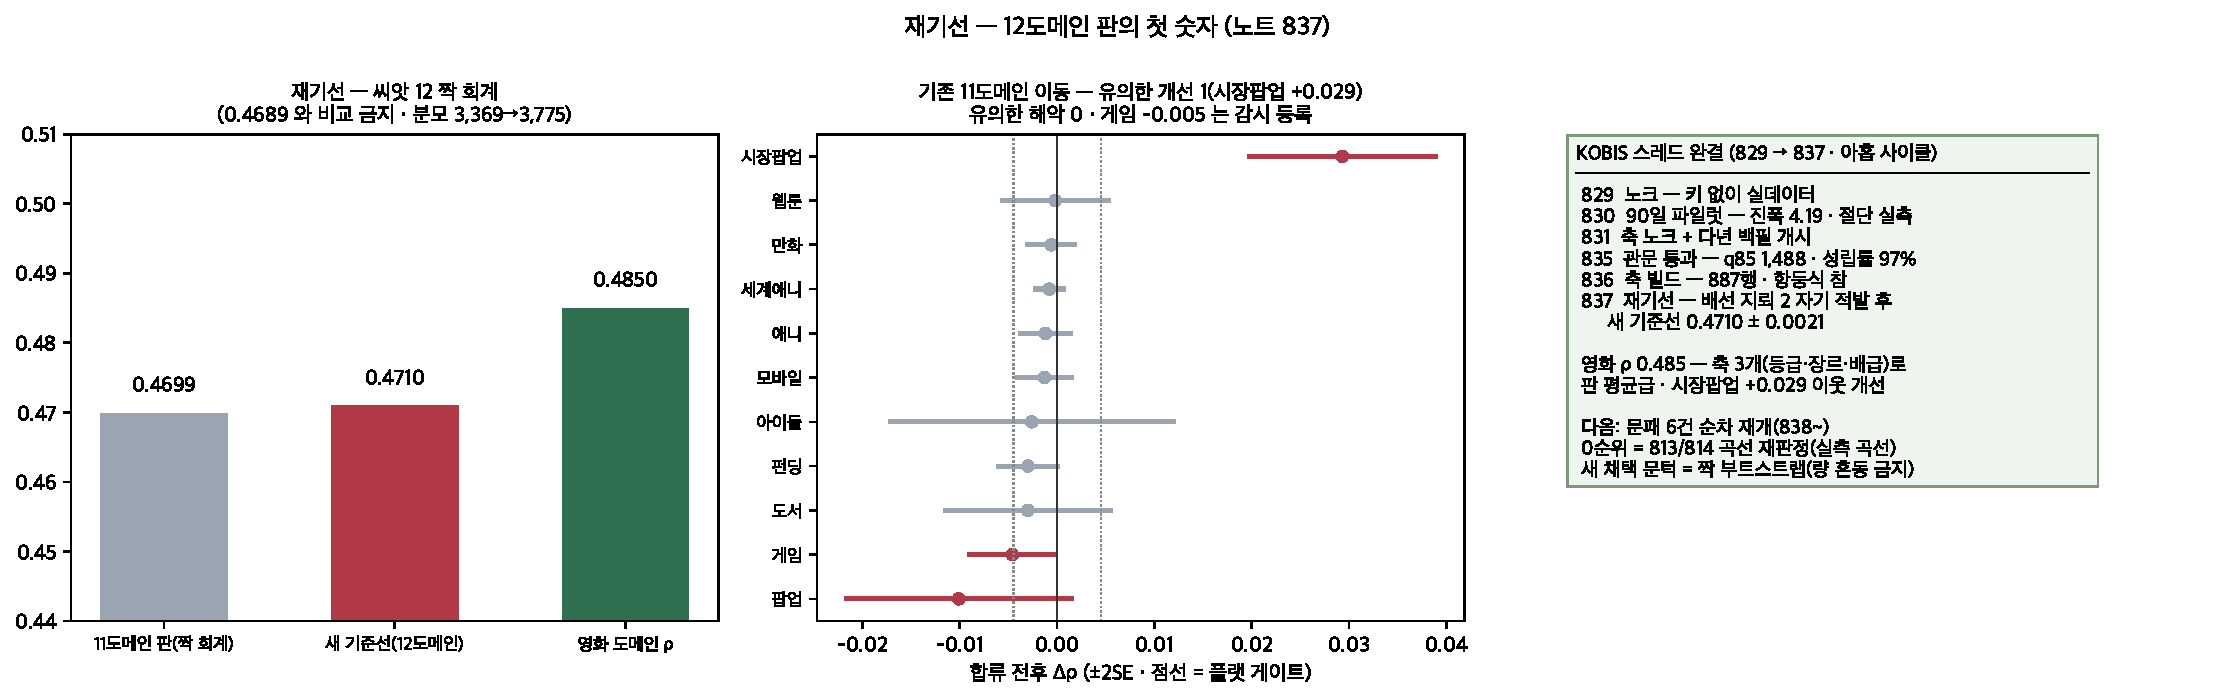
\includegraphics[width=0.99\textwidth]{figs/rebase.pdf}
\caption{왼쪽: 재기선 회계. 가운데: 기존 도메인 이동($\pm 2$SE). 오른쪽:
스레드 요약.}
\end{figure}

\section{지뢰 둘을 스스로 밟고 스스로 적발했다}

\claim{\textbf{① 조용한 교집합 축소}: 영화에 이름 $5$개만 주자
\texttt{axis\_order("common")} 이 공유 축을 $36 \to 5$ 로 무너뜨려 $12$도메인
판이 $0.383$(5축 시대 수준)으로 주저앉았다 --- 노트 $359$(조용한 중립화)의
사촌. 공통 이름 전체 $+$ 마스크 $0$ 열로 수리. \textbf{② 량 혼동 자의 재발
차단}: 부트스트랩 ``새 $2\sigma$ $0.0265$''는 판 \emph{절대 수준}의 표본 SD 로,
채택 문턱이 재는 \emph{짝 팔 $\Delta$} 의 SD($608{\sim}611$ 의 $0.0023$)와
다른 량이다 --- $0.262$ 사가를 반복하지 않도록 명시하고, 새 채택 문턱은 첫
채택 실험에서 짝 부트스트랩으로 재기로 등록했다. 라벨 중심화의 관례
이탈(문안$\neq$코드)도 자기 적발해 $y$ 원값(로더 기본)으로 정정 --- $3$차
시행이 정본이다.}
{이동 게이트 $3$건 발화의 조사: \textbf{시장팝업 $+0.0293$($t \approx +6.2$)
--- 유의한 개선}(영화 $897$ 학습행의 이웃 효과 · 같은 `방문' 물리량) · 게임
$-0.0046$($t \approx -2.1$ · 감시 등록) · 팝업 $-0.0101$($t \approx -1.7$ ·
잡음 경계). 해로운 유의 이동 $0$ $\to$ 진행. 다음: \textbf{문패 $6$건 순차
재개}($838{\sim}$) --- $0$순위는 $813/814$ 곡선 재판정(드디어 실측 곡선으로).
판의 새 숫자: \textbf{$0.4710 \pm 0.0021$}.}

\end{document}
